
%(BEGIN_QUESTION)
% Copyright 2006, Tony R. Kuphaldt, released under the Creative Commons Attribution License (v 1.0)
% This means you may do almost anything with this work of mine, so long as you give me proper credit

A liquid flows into a storage vessel:

$$\includegraphics[width=15.5cm]{i01552x01.eps}$$

Load cells installed on the vessel support legs provide a means of measuring accumulated liquid mass.  A computer logs the gross weight of the vessel at 5 minute intervals:

% No blank lines allowed between lines of an \halign structure!
% I use comments (%) instead, so that TeX doesn't choke.

$$\vbox{\offinterlineskip
\halign{\strut
\vrule \quad\hfil # \ \hfil & 
\vrule \quad\hfil # \ \hfil \vrule \cr
\noalign{\hrule}
%
% First row
Gross weight & Time \cr
%
(pounds) & (hour:minute) \cr
%
\noalign{\hrule}
%
% Another row
1342 & 4:55 \cr
%
\noalign{\hrule}
%
% Another row
2003 & 5:00 \cr
%
\noalign{\hrule}
%
% Another row
2624 & 5:05 \cr
%
\noalign{\hrule}
%
% Another row
3255 & 5:10 \cr
%
\noalign{\hrule}
%
% Another row
3927 & 5:15 \cr
%
\noalign{\hrule}
} % End of \halign 
}$$ % End of \vbox

Calculate the following:

\begin{itemize}
\item{} The mass flow rate of the liquid (in units of pounds per hour) at 5:07 
\vskip 10pt
\item{} The average mass flow rate of the liquid (in units of pounds per hour) since the beginning of the hour
\end{itemize}

\vskip 10pt

\vfil 

\underbar{file i01552}
\eject
%(END_QUESTION)





%(BEGIN_ANSWER)

This is a graded question -- no answers or hints given!

%(END_ANSWER)





%(BEGIN_NOTES)

The mass flow rate at 5:07 may be best estimated by calculating a difference quotient between 5:05 and 5:10:

$$\overline{W} = {\Delta m \over \Delta t} = {3255 \hbox{ lb} - 2624 \hbox{ lb} \over 5:10 - 5:05} = {631 \hbox{ lb} \over 5 \hbox{ min}} = {631 \hbox{ lb} \over 0.0833 \hbox{ hr}} = 7572 \hbox{ lb/hr}$$

\vskip 10pt

The average mass flow rate since the beginning of the hour may be best estimated by calculating a difference quotient between 5:00 and 5:15:

$$\overline{W} = {\Delta m \over \Delta t} = {3927 \hbox{ lb} - 2003 \hbox{ lb} \over 5:15 - 5:00} = {1924 \hbox{ lb} \over 15 \hbox{ min}} = {1924 \hbox{ lb} \over 0.25 \hbox{ hr}} = 7696 \hbox{ lb/hr}$$

\vskip 10pt

If one does not read the question closely, one might mistakenly calculate average mass flow rate for the entire period documented in the table.  This is the result:

$$\overline{W} = {\Delta m \over \Delta t} = {3927 \hbox{ lb} - 1342 \hbox{ lb} \over 5:15 - 4:55} = {2585 \hbox{ lb} \over 20 \hbox{ min}} = {2585 \hbox{ lb} \over 0.3333 \hbox{ hr}} = 7755 \hbox{ lb/hr}$$

%INDEX% Mathematics, calculus: derivative (calculating flow rates from measured volumes at specific times)

%(END_NOTES)


